\chapter{Interoperabilidade Semântica}

Como vimos nos capítulos anteriores, um dos maiores problemas atualmente do governo brasileiro é a falta de capacidade que os sistemas têm de se comunicar. Os motivos são vários entre eles a falta de padronização na hora da disponibilização dos dados. Todos esses conceitos estão altamente relacionados com um outro, a interoperabilidade.
	
Abaixo, segue uma tabela contendo conceitos de interoperabilidade de várias iniciativas pelo mundo:

\begin{table}[H]
\begin{center}
    \begin{tabular}{ | p{12,5cm}  | p{3cm} | }
    \hline
   Interoperabilidade refere-se à capacidade de dois ou mais sistemas computacionais quaisquer de interagir e trocar dados para obter resultados conforme o esperado.& \cite{kamada}. \\ \hline
   Interoperabilidade define um conjunto de procedimentos, definição de dados, padrões técnicos e aspectos de implementação que possibilitam a cooperação administrativa através do intercâmbio de dados (com semântica definida) entre organizações e indivíduos que tem seus processos implementados ou suportados por TIC – Tecnologia da informação e Comunicação. & \cite{spb}. \\ \hline
  Interoperabilidade provê habilidade para trocar informação entre diferentes sistemas e usar de maneira eficiente a informação que foi trocada. & \cite{qualipso}. \\ \hline
   Interoperabilidade se refere à habilidade para combinar diferentes aspectos de diferentes organizações, com o objetivo de interagir em benefício das próprias organizações, através do intercâmbio e compartilhamento de informações e conhecimentos entre seus processos (de negócio) automatizados em sistemas, legados ou não, independente de tecnologias, de linguagens e de plataformas de \emph{software} e \emph{hardware}. & \cite{spb}. \\ \hline
Interoperabilidade é a capacidade de organizações díspares e diferentes interagirem para atingir objetivos comuns, convencionados e vantajosos para todas as partes, envolvendo o partilhamento de informações e conhecimento entre as organizações por intermédio dos processos comerciais existentes, pela troca de dados entre seus respectivos sistemas da tecnologia da informação e comunicação (TIC). & \cite{eif}.\\ \hline
   \end{tabular}
    \caption{Conceitos Sobre Interoperabilidade.}
    \label{tab-interoperabilidade}
\end{center}
\end{table}

O conceito pode parecer simples, mas a discussão que o termo traz sobre todos os aspectos envolvidos bem como a implantação de fato da interoperabilidade, são bastante complexas.

Como descrito em \cite{spb}, as organizações enfrentam grandes desafios em termos de interoperabilidade porque os sistemas que hoje precisam interoperar foram construídos, em épocas diferentes, como entidades independentes e monolíticas. Mas como sabemos, estamos vivendo uma época em que cada vez mais o mundo se globaliza, onde mais e mais processos de negócio vão surgindo, atravessando múltiplos domínios administrativos e organizacionais e tonando os aspectos de interoperabilidade em recursos computacionais fatores competitivos cruciais. 

Dentro desse contexto podemos citar alguns obstáculos que dificultam a interoperabilidade entre os sistemas atuais:

\begin{itemize}
\item A maioria dos sistemas atualmente, principalmente os legados, sofrem falta de uso de padrões de dados, metadados, linguagens e infraestrutura para que esses interoperem;
\item Existi uma certa dificuldade em “evangelizar” o assunto de interoperabilidade entres os diversos atores (gestores, desenvolvedores, clientes ,etc) do sistema, de modo que eles precisam usar padrões desde o início, mesmo que o sistema não interopere com ninguém em sua fase inicial.
\item De acordo com \cite{kamada}, existi um obstáculo que refere-se à necessidade de contornar rapidamente as barreiras políticas e legais entre os atores das diversas esferas e níveis de governos e empresas e as restrições de segurança e sigilo de informações.
\end{itemize}

Em meio desses impasses, o governo federal atua em iniciativas como e-PING para reduzir esses obstáculos.

A arquitetura e-PING – Padrões de Interoperabilidade de Governo Eletrônico – define um conjunto mínimo de premissas, políticas e especificações técnicas que regulamentam a utilização da Tecnologia de Informação e Comunicação (TIC) na interoperabilidade de serviços de Governo Eletrônico, estabelecendo as condições de interação com os demais Poderes e esferas de governo e com a sociedade em geral \cite{eping}.

Os padrões e as políticas contidas no e-PING não são impostas de forma obrigatória para sociedade. No entanto, caso queiramos interoperar com o governo federal, esses padrões e essas políticas devem ser respeitados. 

Para os órgãos do governo federal – Poder Executivo brasileiro – a adoção dos padrões e políticas contidos na e-PING é obrigatória (Portaria SLTI/MP nº 5, de 14 de julho de 2005) \cite{eping}.

Uma dimensão da interoperabilidade importante para o contexto deste trabalho é a interoperabilidade semântica. De acordo com \cite{eif}, interoperabilidade semântica refere-se à habilidade que um sistema deve ter de combinar dinâmica e automaticamente suas informações com outras, recebidas de outros sistemas, e processá-las para produzir determinado valor.	

Para que a interoperabilidade semântica ocorra, é necessário que a interação e a troca de dados entre sistemas estejam livres de ambiguidades, de modo que os dados recebidos por um sistema receptor sejam “entendidos” exatamente como foram enviados pelo sistema emissor.

 Para que isso ocorra, a troca de dados não deve se limitar apenas aos formatos e tipo de dados trocados, mas sobretudo ao conhecimento sobre os dados que devem ser compartilhados entre as partes\cite{kamada}.

Logo, a interoperabilidade semântica trata fundamentalmente da agregação e uso de metadados para “carregar” informações e conhecimento junto aos dados \cite{kamada}.

Fazendo uma correlação com os capítulos anteriores desse trabalho, percebemos que o conceito de interoperabilidade semântica tem uma forte relação com a Web Semântica  e \emph{open linked data\footnote{Linked Data. Disponível em: \url{http://linkedata.org}}}. 

Para \cite{kamada}, toda essa conciliação semântica deve considerar a diversidade de tecnologias, linguagens, ferramentas, ambientes, plataformas operacionais e desenvolvimento de software, novos, legados e futuros, que coexistem nesse grande ecossistema, como representado na figura abaixo:

\graphicspath{{figuras/}}
\begin{figure}[H]
\centering
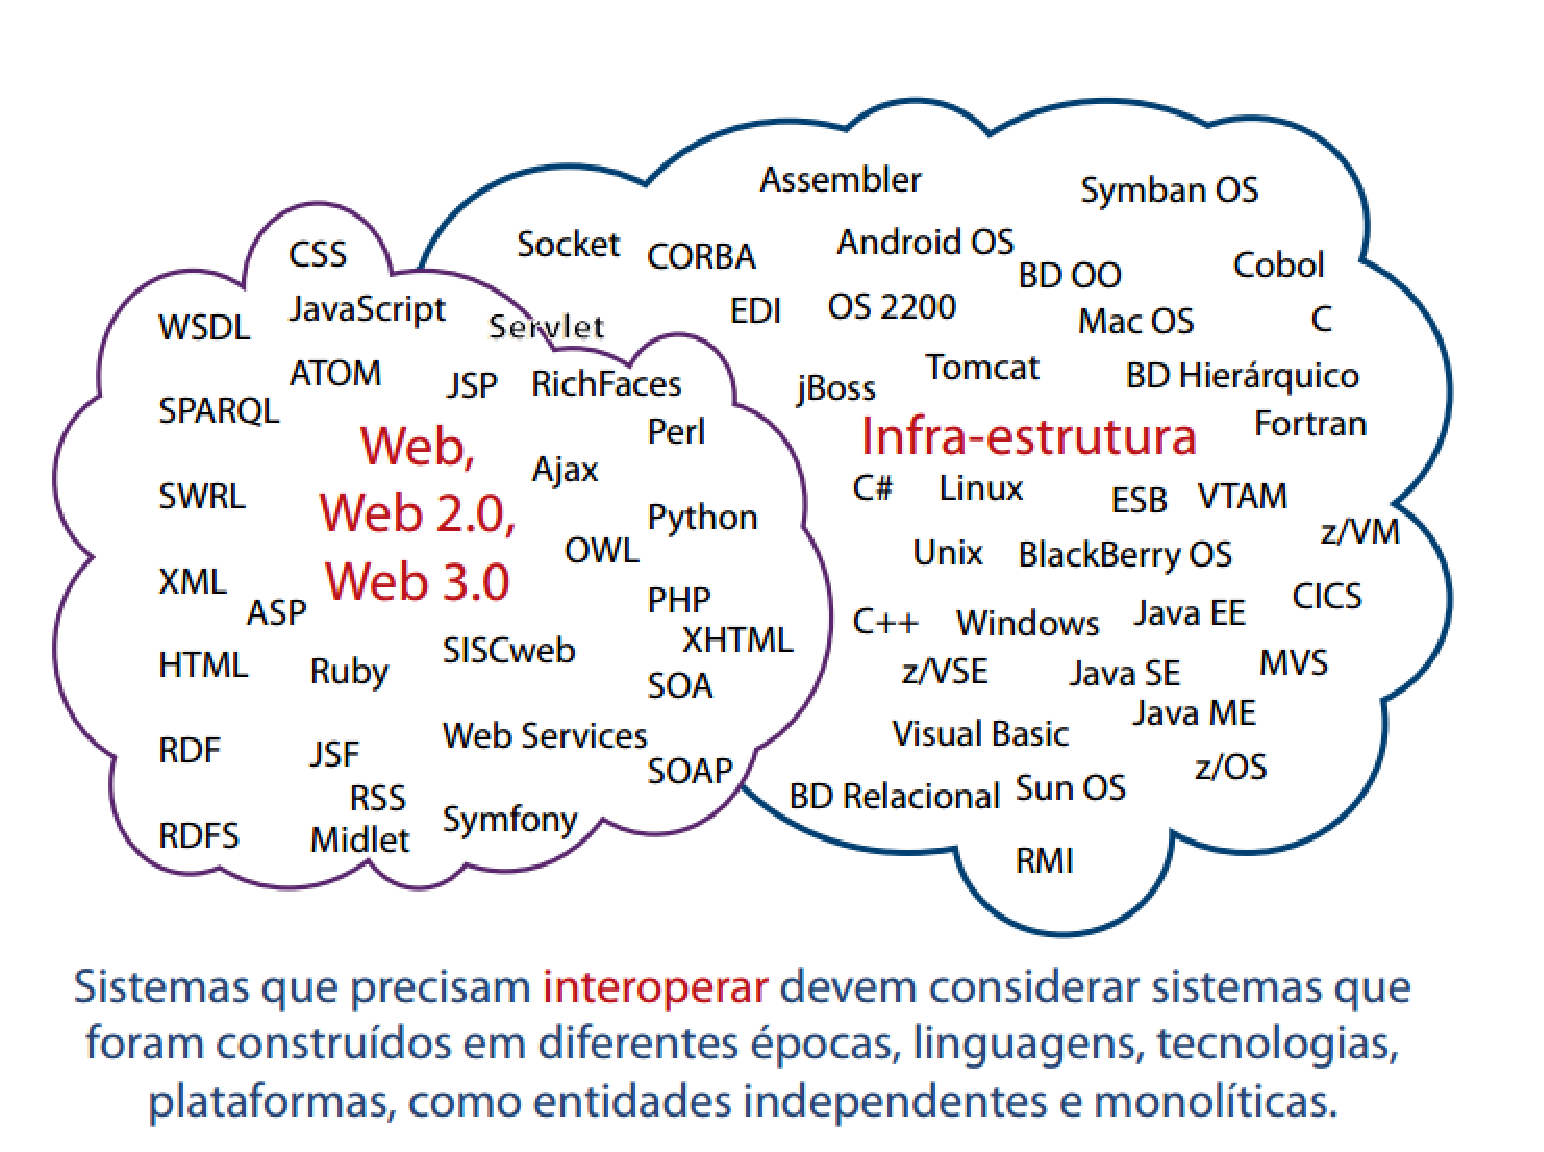
\includegraphics[width=0.8\textwidth]{nuvem_semantica}
\caption[Interoperabilidade considerando a diversidade do ecossistema.]{Interoperabilidade considerando a diversidade do ecossistema. Extraído de \cite{kamada} }
\label{nuvem_semantica}
\end{figure}
Podemos perceber que para conseguir realizar a interoperabilidade semântica devemos resolver um problema que já foi discutido nesse trabalho, a heterogeneidade semântica, que hoje é um dos maiores impasses para integração de sistemas de informação.

Resumindo, a heterogeneidade semântica se deve ao fato de que mudanças de significado que ocorrem, seja dentro de um contexto ao longo do tempo seja por diferenças de requisitos em diferentes domínios, necessariamente resultam em diferentes modelos de informação \cite{kamada}.

De forma geral, temos que conciliar todas essas incompatibilidades semânticas entre os objetos e suas relações nos diferentes domínios, como por exemplo: diferenças de contexto e lógica em esquemas de banco de dados, diferenças entre nomes com mesmos conceitos, entre outros.

Logo, vimos como o conceito de interoperabilidade é importante no contexto do governo federal para promover a cooperação tanto entre os órgãos como sociedade. Podemos afirmar também a necessidade do estabelecimento de políticas de informação que viabilizem a produção e a recepção de informações. Enfim, encarando essas mudanças como uma forma de evolução, futuramente podemos ter um governo mais claro, com uma maior participação da população. 		